\section{Data Description}\label{data}

In this section, we provide a description of the dataset,
followed by an example of a user's data.

\subsection{Dataset}

\change{(M1) Our dataset contains mobile data access history of all active users (during a sunday evening from 6pm to 9pm)
of a major mobile carrier in three cities of China in September 2014. The data was collected by the carrier at the cell tower side.}
For each user, all data request records during the study period are available,
where each record consists of the user ID (a hashed value for anonymity), 
the tower ID (from which we were able to look up its geo-coordinates), 
the timestamp, 
the app identifier, 
and other data access features such as data volumes.

%the following information:
%\begin{description}
%  \item[User ID]: the identifier of a user, a hashed value for anonymity;
%  \item[Tower Location]: the geo-coordinates of a cell phone tower with which a user has established handshake and communicated; %, denoted by $l$.
%  \item[Timestamp]: the Timestamp consists of the date and time of a mobile data access record; %, denoted by $t$.
%  \item[Data Access Features]: contain the app identifier that initiates the data communication, and data volumes.
%  %\item ... represents many other attributes not of focus here.
%\end{description}
%%Note that one app may initiate multiple data transaction records to complete one data transfer in practice, depending on the signal strength and packet deliveries success ratios.

% \begin{figure}[h]
%     \centering
%     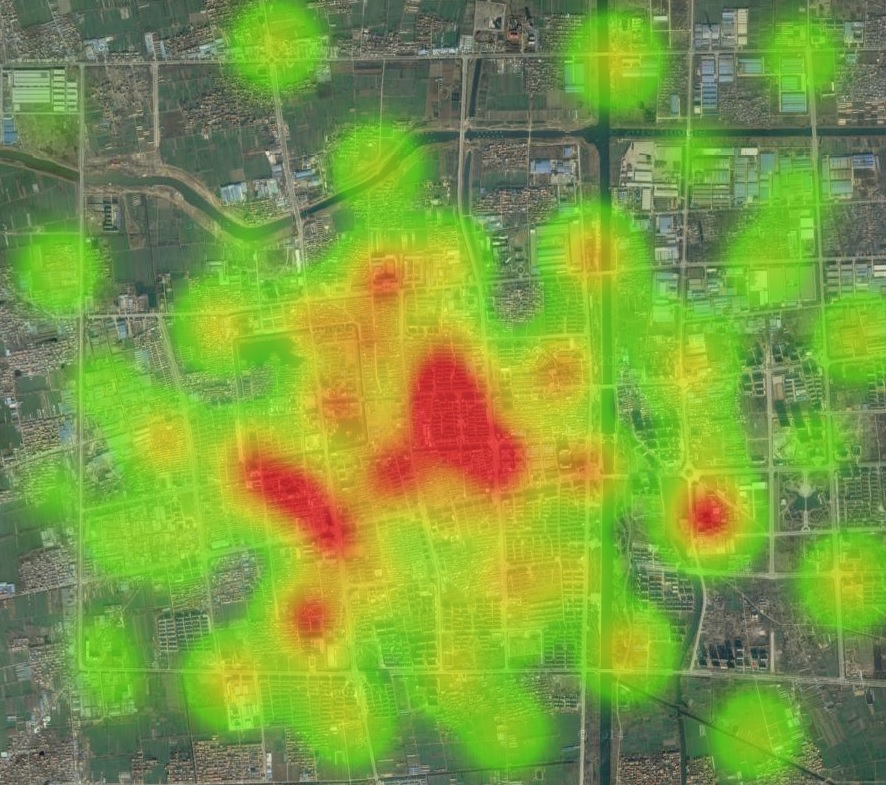
\includegraphics[width=0.6\linewidth]{./figures/hotmap.jpg}
%     %\vspace{-0.1in}
%     \caption{Communication density in a city area.}
%     \label{fig:city_sample} 
%     \vspace{-0.1in}
% \end{figure}

\begin{figure}
\centering
\begin{minipage}{.5\textwidth}
  \centering
  {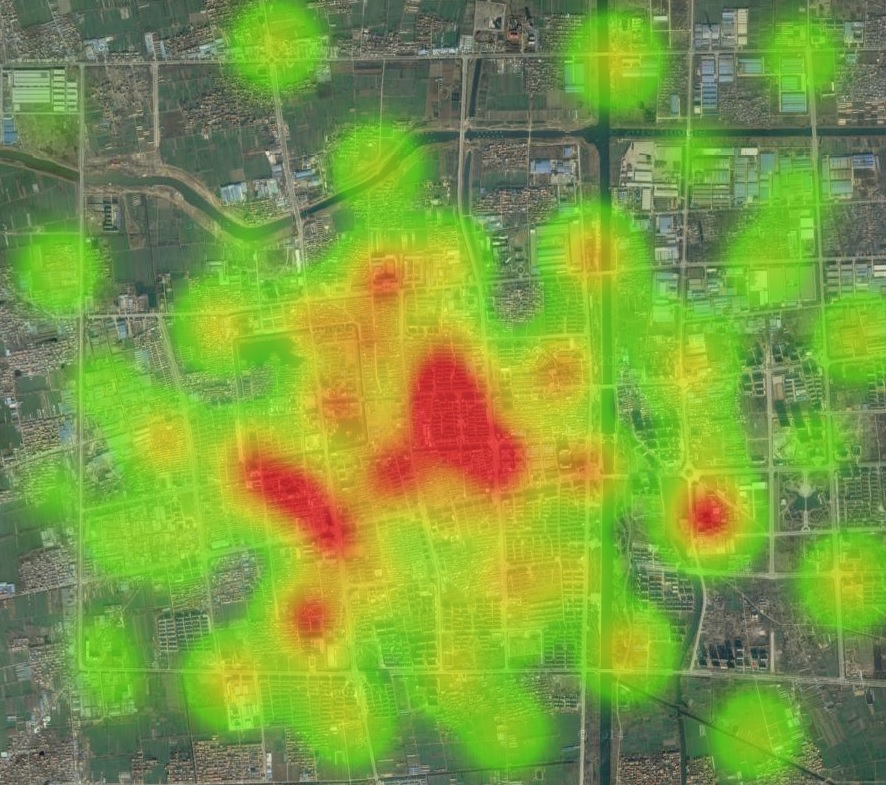
\includegraphics[width=0.915\linewidth]{./figures/hotmap.jpg}}
  \captionof{figure}{Communication density in a city area}
  \label{fig:city_sample}
\end{minipage}%
\begin{minipage}{.5\textwidth}
  \centering
  {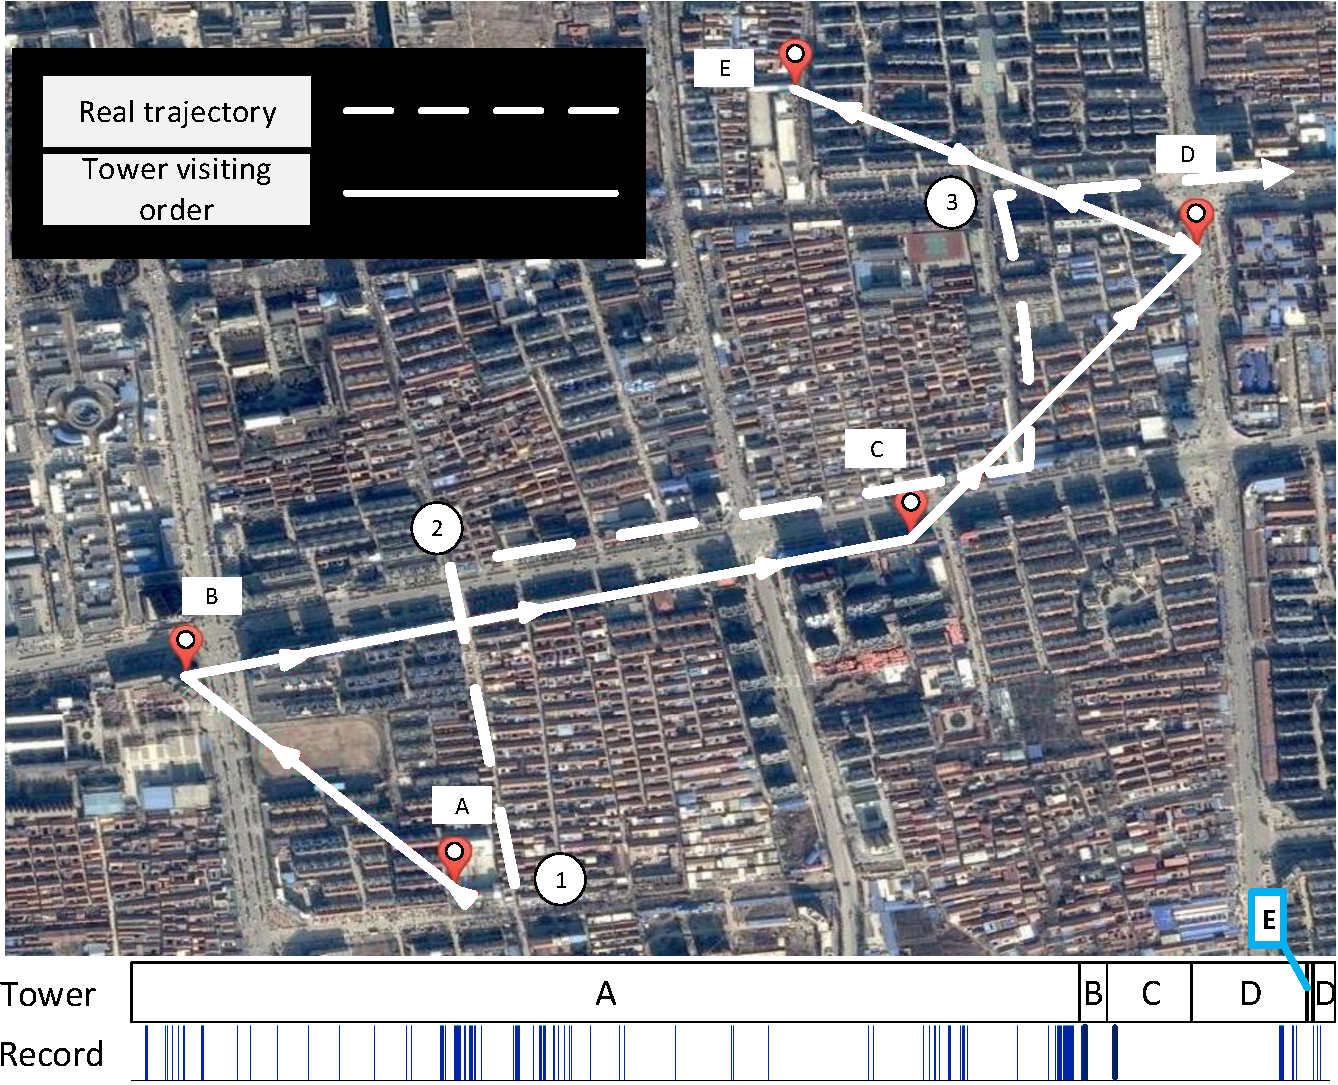
\includegraphics[width=\linewidth]{./figures/typical_user.pdf}}
  \captionof{figure}{Example data access activities of a user}
  \label{fig:typical_user}
\end{minipage}
\end{figure}


%%Before proceeding to the details of our approaches, we briefly introduce our dataset in this section.
%The dataset is a collection of the aforementioned mobile data access records provided by a cellular network operator in China, collected from  three mid-size cities, including both urban and suburban areas, during a three-hour period in the early evening (6pm - 9pm) in 2014. The cities are anonymous in this paper. 
The dataset includes more than 58 million mobile data access records with a total volume of more than 720 gigabytes, which covers all cell phones that were actively exchanging data with a total of 5199 cell towers in the area during the observation period. 
The number of unique users included in this dataset is identified as around 900 thousand. % removing duplicates. 
The total active time of all users accumulates to more than 1 million hours. 
\autoref{fig:city_sample} shows a heatmap of the mobile data access in a city area of our dataset.
The dataset contains both user initiated network access and background network access.

\subsection{Data Preprocessing Findings}

%We first preprocess the dataset and we have the following preliminary findings.
We first preprocess the data and analyze the characteristics of mobile data access patterns.  % of each individual in our study,
Distributional characteristics are visualized in \autoref{fig:data_stat}.
In particular,
the number of records per user,
the average time intervals between consecutive records, and
the number of towers visited.
%the contribution of each category of apps on total mobile data traffic.
We found that our dataset has a highly skewed distribution of
the number of records per user, as shown in \autoref{fig:data_stat1}, and
the time intervals between consecutive records, as shown in \autoref{fig:data_stat2}.
Here, a higher record density, \ie more records for a user in a time unit, indicates a better performance to infer user mobility even when the trip length is very short,
as we can obtain a better granularity by analyzing these records.
Actually, it is the case that most user only traveled a very short trip in terms of the number of visited towers according to \autoref{fig:data_stat3}.

\begin{figure*}
    \centering
    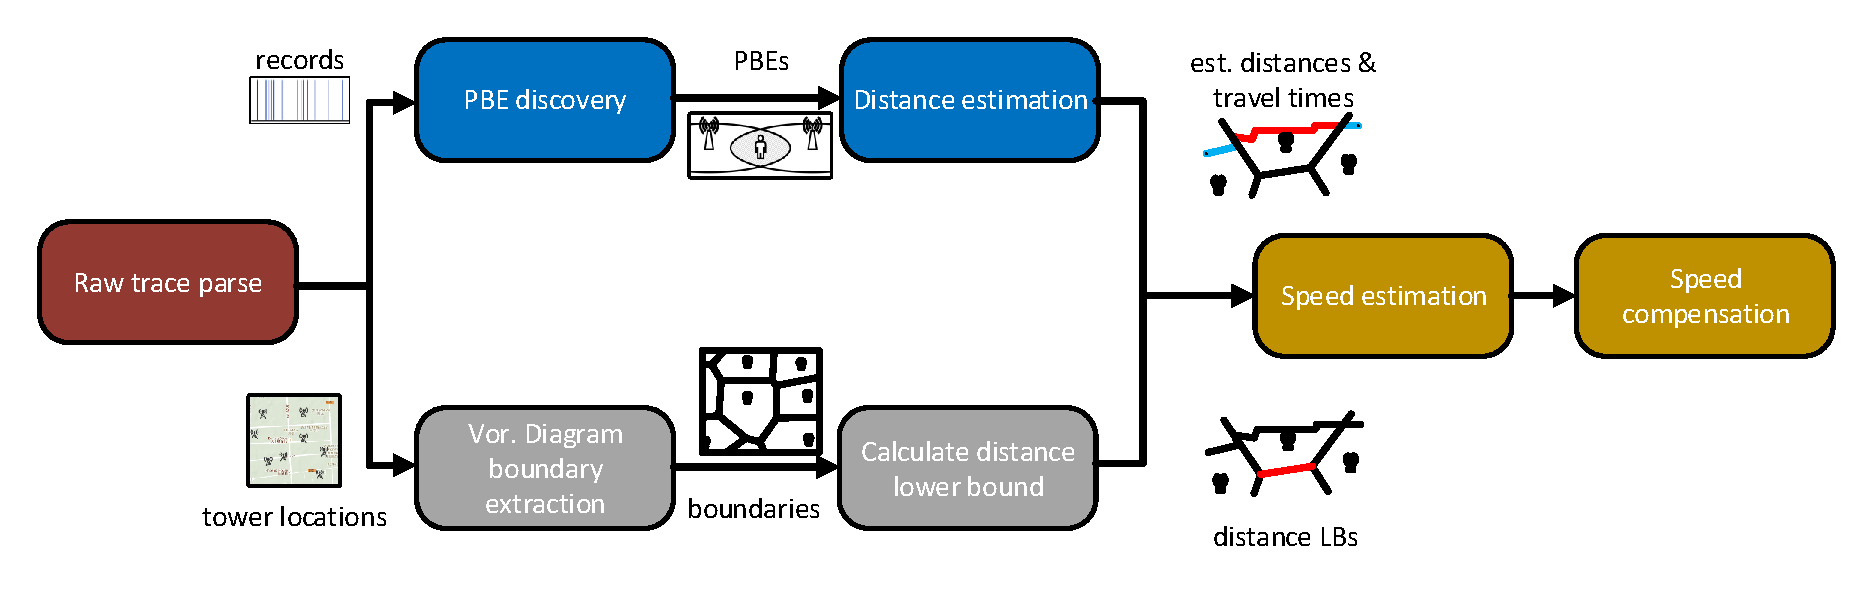
\includegraphics[width=\linewidth]{./figures/system_overview.pdf}
    \vspace{-0.4in}
    \caption{Speed estimation system overview.}
    \label{fig:system_overview}
    \vspace{-0.1in}
\end{figure*}



Note that our dataset differs from commonly used mobility datasets used in existing work.
Compared to moving trajectories like those captured by GPS,
we do not know the exact locations of the users, and we only know a user is located nearby a tower to communicate with it.
Furthermore, compared to other datasets with call detail records (CDR),
our dataset is drawn from a region with more densely populated customers, where each may adopt different mobility methods such as walking, driving, or taking buses.
Such differences make it harder to accurately estimate user speed based on existing methods. %For example...


\subsection{An Example User's Traces}

To provide a clear view of our data, we visualize a user's records from our dataset in \autoref{fig:typical_user} as a running example.

% \begin{figure}[h]
%     \centering
%     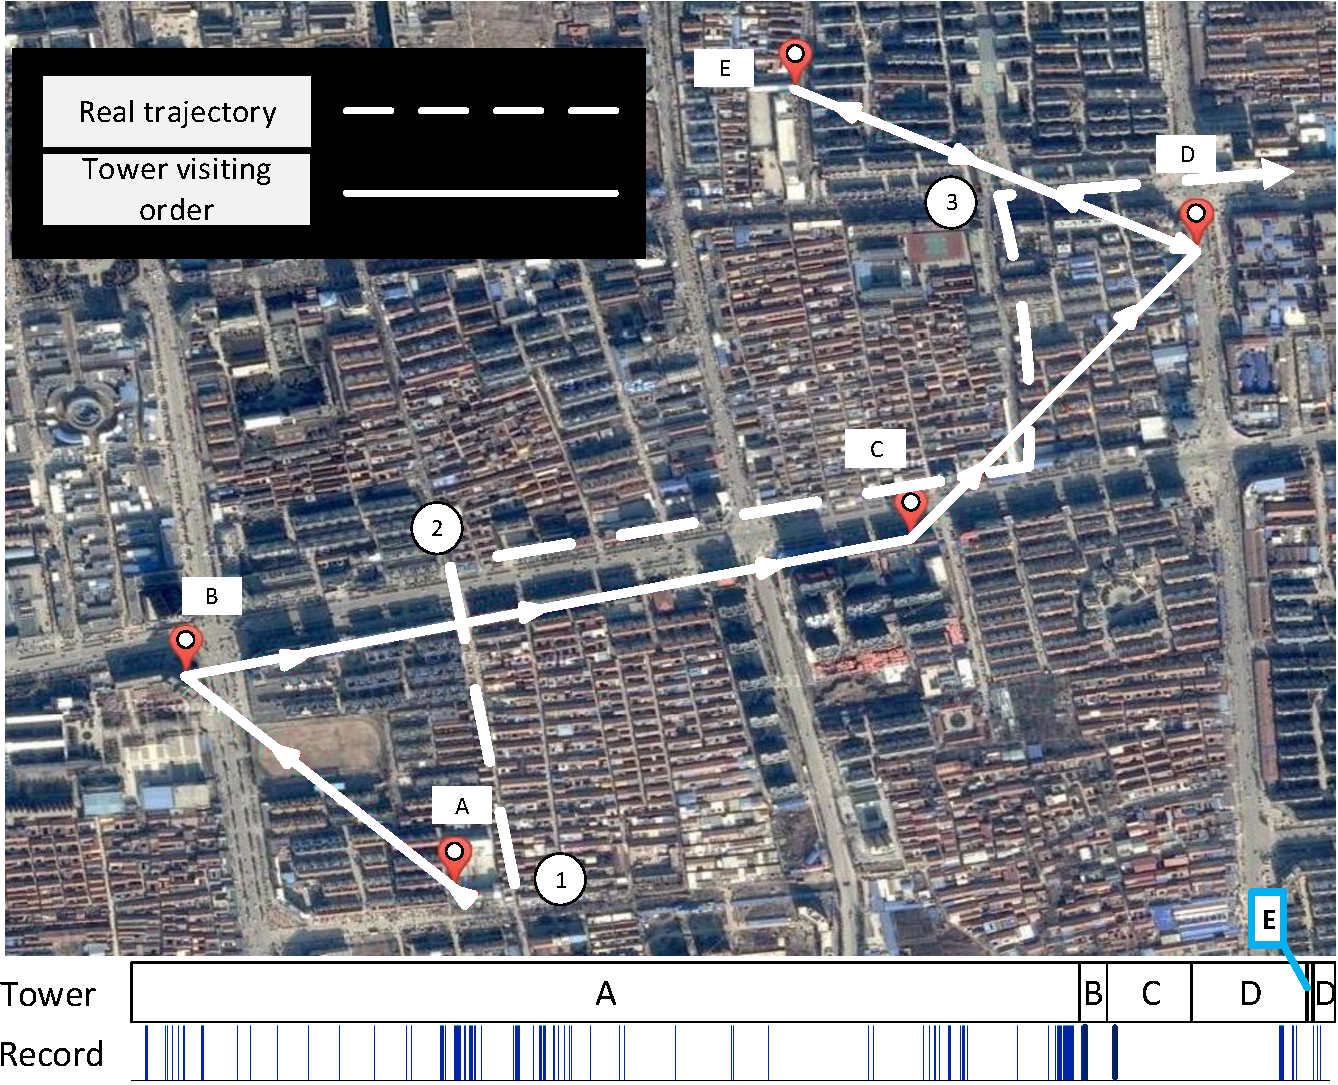
\includegraphics[width=0.8\linewidth]{./figures/typical_user.pdf}
% %     \vspace{-0.3in}
%     \caption{Example data access activities of a user.}
%     \label{fig:typical_user}
%     \vspace{-0.1in}
% \end{figure}

Suppose that the user was taking the path (while using the cell phone) shown with the dashed line.
In particular, she started by walking from location 1, to location 2 where she waited for the bus.
After a few minutes, she got onto the bus, which took the path towards location 3.
Even though we did not know the actual path of the user,
her locations could be inferred by the nearby towers to which her communication data were sent to.


Since the cell tower locations are all known,
we can display the tower locations on a map that were visited by the user.
%Although we do not have the ground truth of user trajectory, for the sake of the example,
We use markers to show tower locations and arrowed lines to show the sequence of visiting.

The bottom part of \autoref{fig:typical_user} shows the timeline of the user's data access records with pulses.
We also show with which tower the user has communicated for each mobile data access record, by providing tower labels above the pulses.
Therefore, for this particular user, she communicated with tower A for a quite long time,
and shortly connected to tower B before switching to tower C.
After a while, the user was found in tower D's coverage area.
Then she connected to tower E for a very short time as location 3 is equally close to both tower C and tower D, \ie a possible cell oscillation, and in the end switched back to tower D.



